
\documentclass[11pt]{article}

% Language setting
\usepackage[turkish]{babel}
\usepackage{pythonhighlight}

\usepackage[a4paper,top=2cm,bottom=2cm,left=2cm,right=2cm,marginparwidth=2cm]{geometry}

% Useful packages
\usepackage{amsmath}
\usepackage{graphicx}
\usepackage[colorlinks=true, allcolors=blue]{hyperref}
\usepackage{verbatim}
\usepackage{fancyhdr} % for header and footer
\usepackage{titlesec}
\usepackage{parskip}

\setlength{\parindent}{0pt}

\titleformat{\subsection}[runin]{\bfseries}{\thesubsection}{1em}{}

\pagestyle{fancy} % activate the custom header/footer

% define the header/footer contents
\lhead{\small{23BLM-4014 Yapay Sinir Ağları Ara Sınav Soru ve Cevap Kağıdı}}
\rhead{\small{Dr. Ulya Bayram}}
\lfoot{}
\rfoot{}

% remove header/footer on first page
\fancypagestyle{firstpage}{
  \lhead{}
  \rhead{}
  \lfoot{}
  \rfoot{\thepage}
}
 

\title{Çanakkale Onsekiz Mart Üniversitesi, Mühendislik Fakültesi, Bilgisayar Mühendisliği Akademik Dönem 2022-2023\\
Ders: BLM-4014 Yapay Sinir Ağları/Bahar Dönemi\\ 
ARA SINAV SORU VE CEVAP KAĞIDI\\
Dersi Veren Öğretim Elemanı: Dr. Öğretim Üyesi Ulya Bayram}
\author{%
\begin{minipage}{\textwidth}
\raggedright
Öğrenci Adı Soyadı: Sarp Ata TÜRKER\\ % Adınızı soyadınızı ve öğrenci numaranızı noktaların yerine yazın
Öğrenci No: 190401015
\end{minipage}%
}

\date{14 Nisan 2023}

\begin{document}
\maketitle

\vspace{-.5in}
\section*{Açıklamalar:}
\begin{itemize}
    \item Vizeyi çözüp, üzerinde aynı sorular, sizin cevaplar ve sonuçlar olan versiyonunu bu formatta PDF olarak, Teams üzerinden açtığım assignment kısmına yüklemeniz gerekiyor. Bu bahsi geçen PDF'i oluşturmak için LaTeX kullandıysanız, tex dosyasının da yer aldığı Github linkini de ödevin en başına (aşağı url olarak) eklerseniz bonus 5 Puan! (Tavsiye: Overleaf)
    \item Çözümlerde ya da çözümlerin kontrolünü yapmada internetten faydalanmak, ChatGPT gibi servisleri kullanmak serbest. Fakat, herkesin çözümü kendi emeğinden oluşmak zorunda. Çözümlerinizi, cevaplarınızı aşağıda belirttiğim tarih ve saate kadar kimseyle paylaşmayınız. 
    \item Kopyayı önlemek için Github repository'lerinizin hiçbirini \textbf{14 Nisan 2023, saat 15:00'a kadar halka açık (public) yapmayınız!} (Assignment son yükleme saati 13:00 ama internet bağlantısı sorunları olabilir diye en fazla ekstra 2 saat daha vaktiniz var. \textbf{Fakat 13:00 - 15:00 arası yüklemelerden -5 puan!}
    \item Ek puan almak için sağlayacağınız tüm Github repository'lerini \textbf{en geç 15 Nisan 2023 15:00'da halka açık (public) yapmış olun linklerden puan alabilmek için!}
    \item \textbf{14 Nisan 2023, saat 15:00'dan sonra gönderilen vizeler değerlendirilmeye alınmayacak, vize notu olarak 0 (sıfır) verilecektir!} Son anda internet bağlantısı gibi sebeplerden sıfır almayı önlemek için assignment kısmından ara ara çözümlerinizi yükleyebilirsiniz yedekleme için. Verilen son tarih/saatte (14 Nisan 2023, saat 15:00) sistemdeki en son yüklü PDF geçerli olacak.
    \item Çözümlerin ve kodların size ait ve özgün olup olmadığını kontrol eden bir algoritma kullanılacaktır. Kopya çektiği belirlenen vizeler otomatikman 0 (sıfır) alacaktır. Bu nedenle çözümlerinizi ve kodlarınızı yukarıda sağladığım gün ve saatlere kadar kimseyle paylaşmayınız.
    \item Bu vizeden alınabilecek en yüksek not 100'dür. Toplam aldığınız puan 100'ü geçerse, aldığınız not 100'e sabitlenecektir.
    \item LaTeX kullanarak PDF oluşturanlar öz geçmişlerine LaTeX bildiklerini de eklemeyi unutmasınlar :)
    \item Bu vizedeki soruların çözümleri ve tex dosyası için istediğiniz kadar sayıda Github repository'si oluşturabilirsiniz. Sadece yukarıda belirttiğim tarihlerde (14 Nisan 2023 saat 15:00 ile 15 Nisan 2023 saat 15:00 arasında) public yapmayı/halka açmayı ve Github profilinizi de öz geçmişinize eklemeyi unutmayın :)
    \item Bilgisayarınıza hiçbir program kurmadan, Overleaf, Google Colab, Kaggle gibi ortamlar üzerinden bu vizeyi tamamlamanız mümkün. İyi çalışmalar!!
\end{itemize}

(Ekstra 5 puan) \url{https://github.com/sarpataturker/yapay_sinir_aglari}

\newpage
\section{(Toplam 10 Puan) Hopfield Networks:}

\subsection{(2 Puan)} \textbf{ChatGPT’ye size Hopfield Network’ler ile ilgili detaylı bilgi vermesini isteyin. Sorduğunuz soruyu, ChatGPT'nin çıkartığı cevabı aşağı koyun. Bu cevapta anlamadığınız terimleri de ChatGPT’ye sorup, sorduğunuz soruları ve ChatGPT’nin verdiği cevapları da sırayla aşağı koyun.}

\textbf{SORU1:} Hopfield Networkler hakkında detaylı bilgi almam gerekiyor? Detaylıca anlatabilir misin?

\textbf{CEVAP:} Hopfield ağları, çeşitli bellek işlemleri için kullanılan bir tür geri beslemeli sinir ağıdır. Bu ağlar, öğrenilmiş bir dizi deseni tanıyabilen ve benzer bir giriş deseni verildiğinde benzer bir desen üreten bir bellek işlevi gerçekleştirir.

Bir Hopfield ağı, nöronlar veya "hücreler" olarak adlandırılan bir dizi elektro-kimyasal işlemci veya hesaplama birimi içerir. Bu nöronlar, girdi verilerini işlemek için birbirleriyle bağlantılıdır. Bu bağlantılar, ağın bellek işlevini sağlayan geri beslemeli bağlantılardır.

Hopfield ağları, nöronların çıkışlarının her bir nöronun girişine de bağlandığı bir geri besleme yapısına sahiptir. Bu geri besleme yapıları, ağın önceki durumlarından gelen bilgileri kullanarak, mevcut girdilerin işlenmesinde önemli bir rol oynar.

Hopfield ağları, eğitim sırasında desenlerin birbirleriyle olan ilişkisini öğrenir ve daha sonra bu desenleri tanımak için kullanır. Bu ağlar, öğrenilen desenleri hatırlamak ve benzer girdileri tanımak için kullanılabilir.

Hopfield ağları, diğer sinir ağlarına kıyasla oldukça basittir ve sınırlı sayıda nöronla çalışır. Ancak, bu ağların bellek işlevleri ve özellikle de asenkronik dinamikleri, önemli bir matematiksel karmaşıklık içerir.

Hopfield ağları, çeşitli uygulamalarda kullanılmaktadır. Bunlar arasında veri sıkıştırma, modelleme ve tanıma gibi konular yer almaktadır. Ayrıca, Hopfield ağları, yapay zeka ve robotik gibi alanlarda da kullanılmaktadır.

\textbf{SORU2:}5. Satırda bahsettiğin asenkronik dinamikler hakkında bilgi verebilir misin?

\textbf{CEVAP:}Hopfield ağlarının asenkronik dinamikleri, nöronların birbirleriyle bağlantılı olduğu ve bağlantıların geri beslemeli olduğu bir sistemde oluşan zaman bağımlı davranışları ifade eder. Asenkronik dinamikler, nöronların etkileşimlerinin doğası ve zamanlaması ile ilgilidir.

Hopfield ağlarında, her nöronun aktivasyonu, diğer nöronların aktivasyonunu etkileyebilir ve bu etki tüm ağa yayılabilir. Bu durum, ağın dinamik davranışlarını etkiler ve özellikle asenkronik olarak çalışırken, nöronların aktivasyon durumları farklı hızlarda ve farklı sıralamalarda değişebilir.

Asenkronik dinamikler, Hopfield ağlarının bellek işlevlerinde önemli bir rol oynar. Örneğin, bellek çarpışması durumunda, ağda birden fazla desenin etkisi altında kalması durumunda, asenkronik dinamikler desenler arasındaki farklılıkları ayırt etmeye yardımcı olabilir. Ayrıca, Hopfield ağlarının asenkronik dinamikleri, birçok farklı sınıflandırma ve tanıma probleminin çözümünde kullanılabilir.

Ancak, asenkronik dinamiklerin doğası ve karmaşıklığı, Hopfield ağlarının analizini ve tasarımını zorlaştırır. Bu nedenle, Hopfield ağlarının performansını artırmak için, özellikle büyük boyutlu ağlarda, çeşitli teknikler ve yaklaşımlar kullanılır.


\subsection{(8 Puan)} \textbf{ChatGPT’nin açıklamalarından ne anladığınızı buraya kendi kelimelerinizle özetleyin. Örneğin ``Hopfield Network nedir? Ne işe yarar? Neden bilmemiz gerekir bunu? Gerçek hayatta kullanılıyor mu?'' gibi. Anlamadığınız kısımlar varsa ve ChatGPT’nin açıklamaları yeterli gelmezse internet dahil farklı kaynaklardan araştırıp, bilgilerin doğruluğunu sorgulamakta serbestsiniz. Konuyu doğru anlayıp anlamamanız puana etki edecektir. Kullandığınız kaynakları da belirtin!}

Hopfield Network nedir sorusunun cevabıyla başlamak gerekirse, geri beslemeli sinir ağı olarak özetleyebiliriz.
Veri sıkıştırma, modelleme ve tanıma gibi konuların yanı sıra yapay zeka ve robotik gibi alanlarda da kullanılan bir tür yapay sinir ağıdır.
Bu yapay sinir ağını bilmemiz gerekir çünkü diğer sinir ağlarına kıyasla daha basittir.
ChatGPT'ye günlük hayatta nerelerde kullanıldığını sorduğumda bana günlük hayatta doğrudan kullanılmadığını ancak veri sıkıştırma algoritmaları, internet üzerinden veri indirme işlemlerinde kullanılmakta olduğunu ve sesli asistan ve akıllı ev sistemleri gibi teknolojilerin bir parçası olarak kullanılmakta olmasıyla birlikte dolaylı olarak hayatımıza etki ettiğinden bahsetti. Internet üzerinden veri indirmede nasıl kullanıldığını anlamak için ne gibi şekilde kullanıldığı hakkında soru yönelttiğimde bana veri indirme işlemlerinde  sıkıştırma algoritmaları olarak kullanıldığını yöneltti.
Yani kısaca Hopfield Ağları doğrudan olmasa bile dolaylı yoldan bizim hayatımıza oldukça fazla alanda etki etmekteymiş. Örneğin Robotik alanında robotların hareketlerini ve kontrolü ile ilgili problemlerin çözümünde, elektrik enerjisi yönetiminde enerjinin tüketiminin azaltılarak daha verimli kullanılması gibi bir çok alanda bizim hayatımıza etki eden bir yapay sinir ağıymış.

\section{(Toplam 10 Puan) Boltzman Machine:}

\subsection{(2 Puan)} \textbf{ChatGPT’ye size Boltzman Machine ilgili detaylı bilgi vermesini isteyin. Sorduğunuz soruyu, ChatGPT'nin çıkartığı cevabı aşağı koyun. Bu cevapta anlamadığınız terimleri de ChatGPT’ye sorup, sorduğunuz soruları ve ChatGPT’nin verdiği cevapları da sırayla aşağı koyun.}

\textbf{SORU1:} Boltzman Machine hakkında bilgi almam gerekiyor. Detaylı bilgi verebilir misin?

\textbf{CEVAP:} Boltzmann Machine (BM) yapay sinir ağları sınıfındadır ve makine öğrenimi alanında kullanılan bir modeldir. İsmi, fizikteki Boltzmann dağılımından gelir ve makine öğrenimindeki temel işlevlerden biri olan olasılıksal dağılımı temsil eder.

BM, çeşitli uygulamalar için kullanılan birçok farklı varyasyonlara sahip olabilir. Ancak genel olarak, BM birçok bağımsız değişken arasındaki bağımlılıkları öğrenmek için kullanılan bir algoritmadır.

BM, iki tip nöron içerir: gizli ve görünür. Gizli nöronlar, verilerin öznitelikleriyle ilgili olarak öğrenilen gizli özellikleri temsil ederken, görünür nöronlar, girdi verilerinin kendilerini temsil eder. BM, bu nöronları birbirine bağlayan ağırlıkları öğrenir ve bir veri örneği girdisi aldığında, BM, ağırlıkları kullanarak olası diğer öznitelikler için tahminler yapar.

BM, makine öğreniminde çeşitli uygulamalara sahip olabilir. Örneğin, BM, özellik öğrenme, veri boyut azaltma, model seçimi ve olasılık hesaplama gibi çeşitli görevler için kullanılabilir. BM, sınıflandırma ve örüntü tanıma gibi uygulamalar için de kullanılabilir.

Sonuç olarak, Boltzmann Machine, öğrenme algoritması olarak kullanılan yapay sinir ağı modelidir. BM, girdi verileri arasındaki bağımlılıkları öğrenmek için kullanılır ve çeşitli makine öğrenimi görevleri için uygulanabilir.

\textbf{SORU2:} Boltzman dağılımı nedir?

\textbf{CEVAP:} Boltzmann dağılımı, istatistik mekaniğindeki bir olasılık dağılımıdır ve termodinamik sistemlerdeki enerji seviyelerinin dağılımını ifade eder. Bu dağılım, bir sistemin belirli bir sıcaklıkta hangi enerji seviyelerinde bulunabileceğini tahmin etmek için kullanılır.

Boltzmann dağılımı, bir sistemin termodinamik potansiyel enerjisi (E) ve sıcaklığı (T) arasındaki bağıntıyı ifade eder ve şu şekilde yazılabilir:

P(E) = (1/Z) * exp(-E/kT)

Burada P(E), sistemin belirli bir enerji seviyesinde bulunma olasılığını ifade eder. Z, partisyon fonksiyonu olarak adlandırılır ve sistemin tüm olası durumlarının toplam sayısını ifade eder. k, Boltzmann sabiti olarak adlandırılır ve doğal logaritmanın tabanıdır.

Boltzmann dağılımı, bir sistemin olası durumlarının sayısını ve bu durumların her birinin olasılığını tahmin etmek için kullanılır. Bu, termodinamik sistemlerdeki moleküllerin hareketlerinin ve enerji seviyelerinin tahmin edilmesinde kullanılan bir yöntemdir.

Boltzmann dağılımı, makine öğrenimi ve yapay zeka gibi alanlarda da kullanılır. Örneğin, bir Boltzmann Makinesi, belirli bir durumda olasılık hesaplama veya girdi verileri arasındaki ilişkilerin öğrenilmesi için Boltzmann dağılımını kullanabilir.


\subsection{(8 Puan)} \textbf{ChatGPT’nin açıklamalarından ne anladığınızı buraya kendi kelimelerinizle özetleyin. Örneğin ``Boltzman Machine nedir? Ne işe yarar? Neden bilmemiz gerekir bunu? Gerçek hayatta kullanılıyor mu?'' gibi. Anlamadığınız kısımlar varsa ve ChatGPT’nin açıklamaları yeterli gelmezse internet dahil farklı kaynaklardan araştırıp, bilgilerin doğruluğunu sorgulamakta serbestsiniz. Konuyu doğru anlayıp anlamamanız puana etki edecektir. Kullandığınız kaynakları da belirtin!}

Temelde Boltzmann Machine(BM) dediğimiz yapay sinir ağı, fizikteki Boltzmann dağılımının temel işlevlerinden olasılık dağılımını temsil ediyormuş. BM birçok bağımsız değişken arasındaki bağımlılıkları öğrenmek ve anlamak için kullanılan bir tür algoritmadır. Bunu da boltzmann dağılımının özelliklerinden birisi olan bir sistemin belirli sıcaklıkta hangi enerji seviyelerinde bulunabileceğini tahmin etme özelliğini kullanarak yapar. İki tip nöron içerir ve bunlardan birisi gizli birisi de görünür nörondur. Gizli nöronlar verilerin öznitelikleriyle ilgili olarak öğrenilen gizli özellikleri temsil ederken, görünür nöronlar girdi verilerinin kendilerini temsil eder. BM ise bu nöronları birbirine bağlayan ağırlıkları öğrenir  ve veri örneği girilirse BM ağırlıkları kullanarak diğer öznitelikler için olası tahminler yapar.  Eğer büyük veri seti ile çalışıyorsanız bilmeniz gereklidir çünkü veri setleri içndeki özelliklerin etkileşimlerini öğrenerek daha iyi sonuçlar elde etmenizi sağlar. 

\section{(Toplam 10 Puan) Markov Assumption ve Markov Chain:}

\subsection{(2 Puan)} \textbf{ChatGPT’ye size Markov assumption ve Markov Chain ilgili detaylı bilgi vermesini isteyin. Sorduğunuz soruyu, ChatGPT'nin çıkartığı cevabı aşağı koyun. Bu cevapta anlamadığınız terimleri de ChatGPT’ye sorup, sorduğunuz soruları ve ChatGPT’nin verdiği cevapları da sırayla aşağı koyun.}

\textbf{SORU1:} Markov Assumption ve Markov Chain nedir detaylı bir  açıklama verebilir misin?

\textbf{CEVAP:} Markov Assumption, bir olayın gelecekteki durumunun, sadece mevcut duruma bağlı olduğunu ve geçmiş durumlardan bağımsız olduğunu varsayar. Başka bir deyişle, Markov Assumption, gelecekteki durumun, sadece mevcut duruma bağlı olduğunu ve geçmiş durumlardan bağımsız olduğunu varsayar. Bu varsayım, çeşitli algoritmaların ve modellerin tasarımında kullanılır.

Markov Chain ise, Markov Assumption'a dayalı bir matematiksel modeldir. Markov Chain, bir dizi durumdan oluşur ve her durumun bir geçiş olasılığı vardır. Markov Chain, bir sürecin zamanla nasıl değiştiğini modellemek için kullanılır. Markov Chain, bir dizi rastgele değişkenlerden oluşur ve her bir değişken, sadece mevcut duruma bağlı olarak belirlenir.

Markov Chain'in birçok uygulaması vardır. Örneğin, finansal piyasalarda fiyat hareketlerini modellerlemede kullanılır. Ayrıca, dil modelleri ve doğal dil işleme (NLP) gibi alanlarda da kullanılır. Markov Chain'in önemli bir özelliği, gelecekteki durumların, sadece mevcut duruma bağlı olduğu için, geçmiş durumların hafızasız olmasıdır. Bu nedenle, Markov Chain, bellek işleme gerektirmeyen ve işlemi basitleştiren bir modeldir.

\textbf{SORU2:} Mevcut duruma bağlı olarak derken gündelik hayattan bilgi verebilir misin?

\textbf{CEVAP:} Elbette! Mevcut duruma bağlılık, önceki durumların veya olayların sonucunun mevcut durumu belirlemede etkisinin olmadığı anlamına gelir. Bu duruma örnek olarak, bir zarın atılması verilebilir. Her zar atışı, önceki atışların sonucunu etkilemez ve sadece mevcut atışa bağlıdır. Örneğin, birinci atışın sonucu 6 ise, ikinci atışın sonucunu etkilemez ve yine 1/6 olasılıkla herhangi bir sayı gelebilir.

Bir başka örnek olarak, bir hava durumu modeli düşünelim. Hava durumunu tahmin etmek için önceki günlerin hava durumu verileri kullanılabilir. Ancak Markov Assumption'a göre, hava durumu tahmini sadece mevcut hava durumu ile ilgilidir ve önceki günlerin hava durumu tahmininde kullanılan veriler, mevcut durumu belirlemede etkili değildir.

Bu örneklerde, mevcut duruma bağlılık, bir sonraki durumun veya olayın sadece mevcut duruma bağlı olduğu anlamına gelir ve önceki durumların sonucunu etkilemediği anlamına gelir.

\subsection{(8 Puan)} \textbf{ChatGPT’nin açıklamalarından ne anladığınızı buraya kendi kelimelerinizle özetleyin. Örneğin ``Markov assumption ve Markov Chain nedir? Ne işe yarar? Neden bilmemiz gerekir bunu? Gerçek hayatta kullanılıyor mu?'' gibi. Anlamadığınız kısımlar varsa ve ChatGPT’nin açıklamaları yeterli gelmezse internet dahil farklı kaynaklardan araştırıp, bilgilerin doğruluğunu sorgulamakta serbestsiniz. Konuyu doğru anlayıp anlamamanız puana etki edecektir. Kullandığınız kaynakları da belirtin!}

Markov assumption dediğimiz şey, temel mantık üzerinde zar atılması gibi bir durum. Bir zarın atılması durumunda bir önceden çıkasn sonucun o an atılan zarın üzerinde etkisinin olmaması gibi anlık olan değerlerin hesaplanması üzerine olan bir durumdur. Günlük hayatta da dil modellerinde, finansal piyasalarda, reklamcılıkta, robotik üzerinde, epidemioloji (hastalıkların yayaılmasını önleme ve tedavi stratejilerinde) gibi yerlerde kullanılmaktadır ve bu da çeşitli alanlarda kullanılabildiğini gösterir. Ancak bunların yanında öğrenmemizi gerektiren temel sebeplerden birisi verilerin ve süreçlerin modellenmesi için önemli bir araç olarak kullanılır ve elimizdeki anlık verilerle düzgünce veri işlemeyi sağlarız. Kaynak olarak sadece ChatGPT kullandım.

\section{(Toplam 20 Puan) Feed Forward:}
 
\begin{itemize}
    \item Forward propagation için, input olarak şu X matrisini verin (tensöre çevirmeyi unutmayın):\\
    $X = \begin{bmatrix}
        1 & 2 & 3\\
        4 & 5 & 6
        \end{bmatrix}$
    Satırlar veriler (sample'lar), kolonlar öznitelikler (feature'lar).
    \item Bir adet hidden layer olsun ve içinde tanh aktivasyon fonksiyonu olsun
    \item Hidden layer'da 50 nöron olsun
    \item Bir adet output layer olsun, tek nöronu olsun ve içinde sigmoid aktivasyon fonksiyonu olsun
\end{itemize}

Tanh fonksiyonu:\\
$f(x) = \frac{exp(x) - exp(-x)}{exp(x) + exp(-x)}$
\vspace{.2in}

Sigmoid fonksiyonu:\\
$f(x) = \frac{1}{1 + exp(-x)}$

\vspace{.2in}
 \textbf{Pytorch kütüphanesi ile, ama kütüphanenin hazır aktivasyon fonksiyonlarını kullanmadan, formülünü verdiğim iki aktivasyon fonksiyonunun kodunu ikinci haftada yaptığımız gibi kendiniz yazarak bu yapay sinir ağını oluşturun ve aşağıdaki üç soruya cevap verin.}
 
\subsection{(10 Puan)} \textbf{Yukarıdaki yapay sinir ağını çalıştırmadan önce pytorch için Seed değerini 1 olarak set edin, kodu aşağıdaki kod bloğuna ve altına da sonucu yapıştırın:}

% Latex'de kod koyabilirsiniz python formatında. Aşağıdaki örnekleri silip içine kendi kodunuzu koyun
\begin{python}
import torch
x = torch.tensor([1,2,3,4,5,6]).reshape(-1,3).float()
# $f(x) = \frac{1}{1 + exp(-x)}$

def sigmoid_activation(x):
    return 1 / (1 + torch.exp(-x))
# $f(x) = \frac{exp(x) - exp(-x)}{exp(x) + exp(-x)}$
def tanh_function(x):
    return ((torch.exp(x)-torch.exp(-x))/(torch.exp(x)+torch.exp(-x)))
torch.manual_seed(1)

weight1 = torch.randn(3,50) 
bias1 = torch.randn(1,50) 

weight2 = torch.randn(50,1)
bias2 = torch.randn(1, 1)

hidden1 = tanh_function(torch.matmul(x,weight1)+bias1)
output1 = sigmoid_activation(torch.matmul(hidden1,weight2)+bias2)

print(output1)
\end{python}

tensor([[0.0498],
        [0.0075]])

\subsection{(5 Puan)} \textbf{Yukarıdaki yapay sinir ağını çalıştırmadan önce Seed değerini öğrenci numaranız olarak değiştirip, kodu aşağıdaki kod bloğuna ve altına da sonucu yapıştırın:}

\begin{python}
torch.manual_seed(190401015)

weight1 = torch.randn(3,50) 
bias1 = torch.randn(1,50) 

weight2 = torch.randn(50,1)
bias2 = torch.randn(1, 1)

hidden1 = tanh_function(torch.matmul(x,weight1)+bias1)
output1 = sigmoid_activation(torch.matmul(hidden1,weight2)+bias2)

print(output1)
\end{python}

tensor([[0.2297],
        [0.6903]])

\subsection{(5 Puan)} \textbf{Kodlarınızın ve sonuçlarınızın olduğu jupyter notebook'un Github repository'sindeki linkini aşağıdaki url kısmının içine yapıştırın. İlk sayfada belirttiğim gün ve saate kadar halka açık (public) olmasın:}
% size ait Github olmak zorunda, bu vize için ayrı bir github repository'si açıp notebook'u onun içine koyun. Kendine ait olmayıp da arkadaşının notebook'unun linkini paylaşanlar 0 alacak.

\url{https://github.com/sarpataturker/yapay_sinir_aglari/tree/main/Feed_Forward}

\section{(Toplam 40 Puan) Multilayer Perceptron (MLP):} 
\textbf{Bu bölümdeki sorularda benim vize ile beraber paylaştığım Prensesi İyileştir (Cure The Princess) Veri Seti parçaları kullanılacak. Hikaye şöyle (soruyu çözmek için hikaye kısmını okumak zorunda değilsiniz):} 

``Bir zamanlar, çok uzaklarda bir ülkede, ağır bir hastalığa yakalanmış bir prenses yaşarmış. Ülkenin kralı ve kraliçesi onu iyileştirmek için ellerinden gelen her şeyi yapmışlar, ancak denedikleri hiçbir çare işe yaramamış.

Yerel bir grup köylü, herhangi bir hastalığı iyileştirmek için gücü olduğu söylenen bir dizi sihirli malzemeden bahsederek kral ve kraliçeye yaklaşmış. Ancak, köylüler kral ile kraliçeyi, bu malzemelerin etkilerinin patlayıcı olabileceği ve son zamanlarda yaşanan kuraklıklar nedeniyle bu malzemelerden sadece birkaçının herhangi bir zamanda bulunabileceği konusunda uyarmışlar. Ayrıca, sadece deneyimli bir simyacı bu özelliklere sahip patlayıcı ve az bulunan malzemelerin belirli bir kombinasyonunun prensesi iyileştireceğini belirleyebilecekmiş.

Kral ve kraliçe kızlarını kurtarmak için umutsuzlar, bu yüzden ülkedeki en iyi simyacıyı bulmak için yola çıkmışlar. Dağları tepeleri aşmışlar ve nihayet "Yapay Sinir Ağları Uzmanı" olarak bilinen yeni bir sihirli sanatın ustası olarak ün yapmış bir simyacı bulmuşlar.

Simyacı önce köylülerin iddialarını ve her bir malzemenin alınan miktarlarını, ayrıca iyileşmeye yol açıp açmadığını incelemiş. Simyacı biliyormuş ki bu prensesi iyileştirmek için tek bir şansı varmış ve bunu doğru yapmak zorundaymış. (Original source: \url{https://www.kaggle.com/datasets/unmoved/cure-the-princess})

(Buradan itibaren ChatGPT ve Dr. Ulya Bayram'a ait hikayenin devamı)

Simyacı, büyülü bileşenlerin farklı kombinasyonlarını analiz etmek ve denemek için günler harcamış. Sonunda birkaç denemenin ardından prensesi iyileştirecek çeşitli karışım kombinasyonları bulmuş ve bunları bir veri setinde toplamış. Daha sonra bu veri setini eğitim, validasyon ve test setleri olarak üç parçaya ayırmış ve bunun üzerinde bir yapay sinir ağı eğiterek kendi yöntemi ile prensesi iyileştirme ihtimalini hesaplamış ve ikna olunca kral ve kraliçeye haber vermiş. Heyecanlı ve umutlu olan kral ve kraliçe, simyacının prensese hazırladığı ilacı vermesine izin vermiş ve ilaç işe yaramış ve prenses hastalığından kurtulmuş.

Kral ve kraliçe, kızlarının hayatını kurtardığı için simyacıya krallıkta kalması ve çalışmalarına devam etmesi için büyük bir araştırma bütçesi ve çok sayıda GPU'su olan bir server vermiş. İyileşen prenses de kendisini iyileştiren yöntemleri öğrenmeye merak salıp, krallıktaki üniversitenin bilgisayar mühendisliği bölümüne girmiş ve mezun olur olmaz da simyacının yanında, onun araştırma grubunda çalışmaya başlamış. Uzun yıllar birlikte krallıktaki insanlara, hayvanlara ve doğaya faydalı olacak yazılımlar geliştirmişler, ve simyacı emekli olduğunda prenses hem araştırma grubunun hem de krallığın lideri olarak hayatına devam etmiş.

Prenses, kendisini iyileştiren veri setini de, gelecekte onların izinden gidecek bilgisayar mühendisi prensler ve prensesler başkalarına faydalı olabilecek yapay sinir ağları oluşturmayı öğrensinler diye halka açmış ve sınavlarda kullanılmasını salık vermiş.''

\textbf{İki hidden layer'lı bir Multilayer Perceptron (MLP) oluşturun beşinci ve altıncı haftalarda yaptığımız gibi. Hazır aktivasyon fonksiyonlarını kullanmak serbest. İlk hidden layer'da 100, ikinci hidden layer'da 50 nöron olsun. Hidden layer'larda ReLU, output layer'da sigmoid aktivasyonu olsun.}

\textbf{Output layer'da kaç nöron olacağını veri setinden bakıp bulacaksınız. Elbette bu veriye uygun Cross Entropy loss yöntemini uygulayacaksınız. Optimizasyon için Stochastic Gradient Descent yeterli. Epoch sayınızı ve learning rate'i validasyon seti üzerinde denemeler yaparak (loss'lara overfit var mı diye bakarak) kendiniz belirleyeceksiniz. Batch size'ı 16 seçebilirsiniz.}

\subsection{(10 Puan)} \textbf{Bu MLP'nin pytorch ile yazılmış class'ının kodunu aşağı kod bloğuna yapıştırın:}

\begin{python}
class MLP(nn.Module):
    def __init__(self, insize, hidden1, hidden2, outputsize):
        super(MLP, self).__init__()
        self.hidden_layer1 = nn.Linear(insize, hidden1)
        self.hidden_layer2 = nn.Linear(hidden1, hidden2)
        self.output_layer = nn.Linear(hidden2, outputsize)
        self.relu = nn.ReLU()
        self.sigmoid = nn.Sigmoid()

    def forward(self, x):
        output = self.relu(self.hidden_layer1(x))
        output = self.relu(self.hidden_layer2(output))
        output = self.sigmoid(self.output_layer(output))
        return output
\end{python}

\subsection{(10 Puan)} \textbf{SEED=öğrenci numaranız set ettikten sonra altıncı haftada yazdığımız gibi training batch'lerinden eğitim loss'ları, validation batch'lerinden validasyon loss değerlerini hesaplayan kodu aşağıdaki kod bloğuna yapıştırın ve çıkan figürü de alta ekleyin.}

\begin{python}
import time
start = time.time()
import torch
import torch.nn as nn
import torch.optim as optim
from torch.utils.data import Dataset, DataLoader, TensorDataset
from sklearn.metrics import accuracy_score, precision_score, recall_score, f1_score
from sklearn.preprocessing import MultiLabelBinarizer
import pandas as pd
import numpy as np
import os
torch.manual_seed(190401015)
class MLP(nn.Module):
    def __init__(self, insize, hidden1, hidden2, outputsize):
        super(MLP, self).__init__()
        self.hidden_layer1 = nn.Linear(insize, hidden1)
        self.hidden_layer2 = nn.Linear(hidden1, hidden2)
        self.output_layer = nn.Linear(hidden2, outputsize)
        self.relu = nn.ReLU()
        self.sigmoid = nn.Sigmoid()

    def forward(self, x):
        output = self.relu(self.hidden_layer1(x))
        output = self.relu(self.hidden_layer2(output))
        output = self.sigmoid(self.output_layer(output))
        return output
training_data = pd.read_csv("./cure_the_princess_train.csv")
val_data = pd.read_csv("./cure_the_princess_validation.csv")
test_data = pd.read_csv("./cure_the_princess_test.csv")
labels = training_data.columns.tolist()
num_of_classes = len(labels)
train_x = training_data.iloc[:, :-1].values
train_y = training_data.iloc[:, -1].values
val_x = val_data.iloc[:, :-1].values
val_y = val_data.iloc[:, -1].values
test_x = test_data.iloc[:, :-1].values
test_y = test_data.iloc[:, -1].values
class CustomData(Dataset):
    def __init__(self, x, y):
        self.x = torch.tensor(x, dtype=torch.float32)
        self.y = torch.tensor(y, dtype=torch.long)

    def __len__(self):
        return len(self.x)

    def __getitem__(self, idx):
        return self.x[idx], self.y[idx]

train_data = CustomData(train_x, train_y)
validation_data = CustomData(val_x, val_y)
test_data = CustomData(test_x, test_y)

learning_rate = 0.00167
epochnum = 200
bsize = 16
insize = 13
hidden1 = 100
hidden2 = 50
outsize = 1
patience = 10
model = MLP(insize, hidden1, hidden2, outsize)
# Loss fonksiyonunu belirlemek / Determining loss function
criterion = nn.BCELoss()

# Optimizer'ı belirlemek / Determining optimizer
optimizer = optim.SGD(model.parameters(), lr=learning_rate)
train_loader = torch.utils.data.DataLoader(train_data, batch_size=bsize, shuffle=True)
valid_loader = torch.utils.data.DataLoader(validation_data, batch_size=bsize, shuffle=False)
test_loader = torch.utils.data.DataLoader(test_data, batch_size=bsize, shuffle=False)
train_loss_list = []
valid_loss_list = []
patience_counter = 0
best_value_loss = None
for epoch in range(epochnum):
    train_loss = 0.0
    train_count = 0.0
    valid_loss = 0.0

    # Eğitim verileri üzerinde eğitim yapmak / Training
    for data, target in train_loader:
        optimizer.zero_grad()
        output = model(data)
        loss = criterion(output, target.unsqueeze(1).float())
        loss.backward()
        optimizer.step()
        train_count += 1
        train_loss += loss.item()

    # Doğrulama verileri üzerinde test yapmak / Testing
    with torch.no_grad():
        model.eval()
        for data, target in valid_loader:
            output = model(data)
            loss = criterion(output, target.unsqueeze(1).float())
            valid_loss += loss.item()
    
    model.train()
    # Loss değerlerini kaydetmek / Saving the Loss values
    train_loss = train_loss / train_count
    valid_loss = valid_loss / len(valid_loader)
        
    train_loss_list.append(train_loss)
    valid_loss_list.append(valid_loss)
    print('Epoch: {} \tTraining Loss: {:.6f} \tValidation Loss: {:.6f}'.format(
        epoch + 1, train_loss, valid_loss))
    
    val_score = valid_loss
    if best_value_loss is None:
        best_value_loss = val_score # hafızada patience boyu tutmaya başla
        torch.save(model.state_dict(), "checkpoint.pt")
    elif best_value_loss < val_score: # patience counter
        patience_counter = patience_counter + 1
        print("Earlystopping Patience Counter:",patience_counter)
        if patience_counter == patience:
            break
    else:
        best_value_loss = val_score
        torch.save(model.state_dict(), "checkpoint.pt") # to keep the best model
        patience_counter = 0

import seaborn as sns
import matplotlib.pyplot as plt

sns.set_style("whitegrid")
plt.plot(train_loss_list, label="Training loss")
plt.plot(valid_loss_list, label="Validation loss")
plt.xlabel("Epoch")
plt.ylabel("Loss")
plt.legend()
plt.show()

from sklearn.metrics import accuracy_score, f1_score, precision_score, recall_score

model.load_state_dict(torch.load('checkpoint.pt'))

preds = []
tlabels = []
model.eval()
with torch.no_grad():
    for inputs, labels in test_loader:
        outputs = model(inputs)
        predicted = torch.round(outputs)
        preds.extend(predicted.detach().cpu().numpy())
        tlabels.extend(labels.detach().cpu().numpy())

accuracy = accuracy_score(tlabels, preds)
f1 = f1_score(tlabels, preds)
precision = precision_score(tlabels, preds)
recall = recall_score(tlabels, preds)

print(f'Accuracy: {accuracy:.4f}')
print(f'F1 score: {f1:.4f}')
print(f'Precision: {precision:.4f}')
print(f'Recall: {recall:.4f}')

end = time.time()
elapsed = end - start
print("Elapsed:", f'{elapsed:.2f}', "secs")
\end{python}

% Figure aşağıda comment içindeki kısımdaki gibi eklenir.

\begin{figure}[ht!]
    \centering
    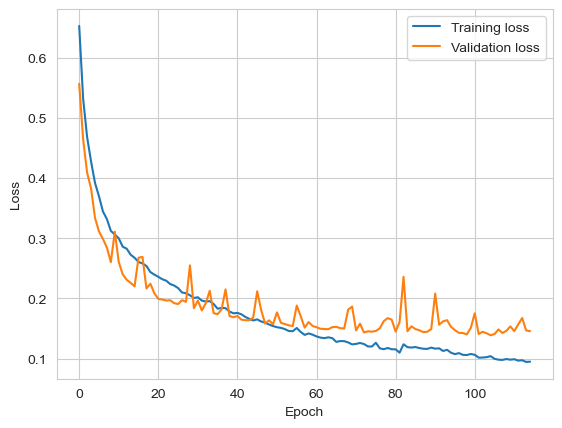
\includegraphics{plotoutput.png}
    \caption{Plot çıktısı}
    \label{fig:my_pic}
\end{figure}


\subsection{(10 Puan)} \textbf{SEED=öğrenci numaranız set ettikten sonra altıncı haftada ödev olarak verdiğim gibi earlystopping'deki en iyi modeli kullanarak, Prensesi İyileştir test setinden accuracy, F1, precision ve recall değerlerini hesaplayan kodu yazın ve sonucu da aşağı yapıştırın. \%80'den fazla başarı bekliyorum test setinden. Daha düşükse başarı oranınız, nerede hata yaptığınızı bulmaya çalışın. \%90'dan fazla başarı almak mümkün (ben denedim).}

\begin{python}

learning_rate = 0.0002786
epochnum = 2000
bsize = 16
insize = 13
hidden1 = 100
hidden2 = 50
outsize = 1
patience = 10

patience_counter = 0
best_value_loss = None
for epoch in range(epochnum):
    train_loss = 0.0
    train_count = 0.0
    valid_loss = 0.0

    # Eğitim verileri üzerinde eğitim yapmak / Training
    for data, target in train_loader:
        optimizer.zero_grad()
        output = model(data)
        loss = criterion(output, target.unsqueeze(1).float())
        loss.backward()
        optimizer.step()
        train_count += 1
        train_loss += loss.item()

    # Doğrulama verileri üzerinde test yapmak / Testing
    with torch.no_grad():
        model.eval()
        for data, target in valid_loader:
            output = model(data)
            loss = criterion(output, target.unsqueeze(1).float())
            valid_loss += loss.item()
    
    model.train()
    # Loss değerlerini kaydetmek / Saving the Loss values
    train_loss = train_loss / train_count
    valid_loss = valid_loss / len(valid_loader)
        
    train_loss_list.append(train_loss)
    valid_loss_list.append(valid_loss)
    print('Epoch: {} \tTraining Loss: {:.6f} \tValidation Loss: {:.6f}'.format(
        epoch + 1, train_loss, valid_loss))
    
    val_score = valid_loss
    if best_value_loss is None:
        best_value_loss = val_score # hafızada patience boyu tutmaya başla
        torch.save(model.state_dict(), "checkpoint.pt")
    elif best_value_loss < val_score: # patience counter
        patience_counter = patience_counter + 1
        print("Earlystopping Patience Counter:",patience_counter)
        #if patience_counter == patience:
        #    break
    else:
        best_value_loss = val_score
        torch.save(model.state_dict(), "checkpoint.pt") # to keep the best model
        patience_counter = 0
\end{python}

\subsection{(5 Puan)} \textbf{Tüm kodların CPU'da çalışması ne kadar sürüyor hesaplayın. Sonra to device yöntemini kullanarak modeli ve verileri GPU'ya atıp kodu bir de böyle çalıştırın ve ne kadar sürdüğünü hesaplayın. Süreleri aşağıdaki tabloya koyun. GPU için Google Colab ya da Kaggle'ı kullanabilirsiniz, iki ortam da her hafta saatlerce GPU hakkı veriyor.}

\begin{table}[ht!]
    \centering
    \caption{100 epoch && batchsize =16}
    \begin{tabular}{c|c}
        Ortam & Süre (saniye) \\\hline
        CPU & 3.04 secs\\
        GPU & 23.09 secs\\
    \end{tabular}
    \label{tab:my_table}
\end{table}

\subsection{(3 Puan)} \textbf{Modelin eğitim setine overfit etmesi için elinizden geldiği kadar kodu gereken şekilde değiştirin, validasyon loss'unun açıkça yükselmeye başladığı, training ve validation loss'ları içeren figürü aşağı koyun ve overfit için yaptığınız değişiklikleri aşağı yazın. Overfit, tam bir çanak gibi olmalı ve yükselmeli. Ona göre parametrelerle oynayın.}

Cevaplar buraya

% Figür aşağı
\begin{figure}[ht!]
    \centering
    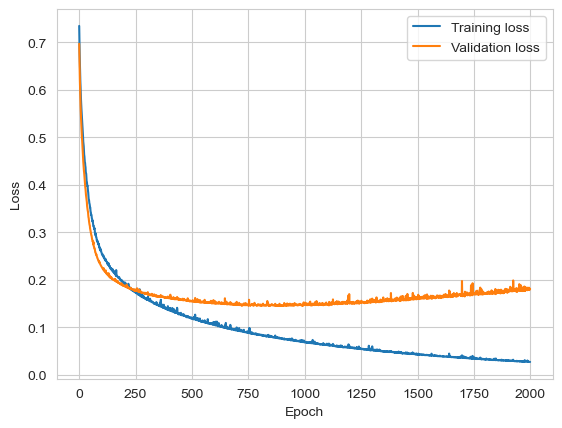
\includegraphics{plot.png}
    \caption{Plot çıktısı}
    \label{fig:my_pic}
\end{figure}

\subsection{(2 Puan)} \textbf{Beşinci soruya ait tüm kodların ve cevapların olduğu jupyter notebook'un Github linkini aşağıdaki url'e koyun.}

\url{https://github.com/sarpataturker/yapay_sinir_aglari/tree/main/MLP}
\pagebreak
\section{(Toplam 10 Puan)} \textbf{Bir önceki sorudaki Prensesi İyileştir problemindeki yapay sinir ağınıza seçtiğiniz herhangi iki farklı regülarizasyon yöntemi ekleyin ve aşağıdaki soruları cevaplayın.} 

\subsection{(2 puan)} \textbf{Kodlarda regülarizasyon eklediğiniz kısımları aşağı koyun:} 

\begin{python}
kod_buraya = None
if kod_buraya:
    devam_ise_buraya = 0

print(devam_ise_buraya)
\end{python}

\subsection{(2 puan)} \textbf{Test setinden yeni accuracy, F1, precision ve recall değerlerini hesaplayıp aşağı koyun:}

Sonuçlar buraya.

\subsection{(5 puan)} \textbf{Regülarizasyon yöntemi seçimlerinizin sebeplerini ve sonuçlara etkisini yorumlayın:}

Yorumlar buraya.

\subsection{(1 puan)} \textbf{Sonucun github linkini  aşağıya koyun:}

\url{www.benimgithublinkim2.com}

\end{document}